\chapter{Využití symetrie}

Operátory pracující s poli jsou definovány tak, že nezávisí na soustavě souřadnic, a proto zachovávají symetrii. Proto pokud máme parciální diferenciální rovnici, která je definovaná pomocí
těchto operátorů, její zdroje jsou symetricky rozloženy a i okrajové podmínky jsou symetrické, pak musí být symetrické i řešení této rovnice. To nám umožňuje v některých případech
řešit rovnice poměrně jednoduše analyticky. Fyzikální interpretace této skutečnosti je, že vesmír nemá žádný souřadnicový systém, ten je pouze myšlený. Proto řešení rovnice, která popisuje
nějaký fyzikální proces, nemůže záviset na volbě souřadnicového systému. Je-li konfigurace fyzikálních objektů symetrická, pak zde neexistuje nic, co by zapřičinilo porušení této symetrie
v řešení rovnice.

V této kapitole odvodíme potenciál kruhového disku v rovině a koule v prostoru. Budeme je potřebovat pro výpočet potenciálu bodového zdroje, který je nutný znát pro řešení Poissonovy rovnice
bez okrajových podmínek. Dále si spíše ze zajímavosti odvodíme indukčnost toroidní cívky.

\section{Potenciál kruhového disku v rovině}

Mějme kruhový disk o~poloměru \(R\) s konstantním buzením \(f\). Chceme vypočítat potenciál \(\varphi\). Konfigurace je rotačně symetrická vůči středu
disku, proto i řešení rovnice je rotačně symetrické. Potenciál proto závisí pouze na vzdálenosti od středu disku \(r\).


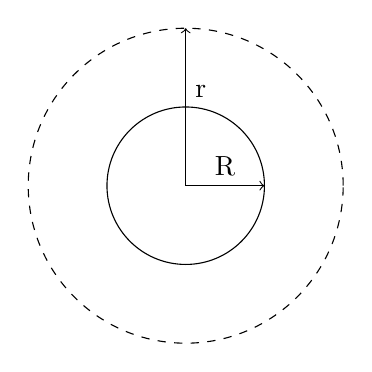
\begin{tikzpicture}
\draw (0, 0) circle(1);
\draw[->] (0, 0) -- (1, 0);
\draw (0.5, 0) node[anchor=south]{R};

\draw[dashed] (0, 0) circle(2);
\draw[->] (0, 0) -- (0, 2);
\draw (0, 1) node[anchor=south west]{r};

\end{tikzpicture}


\begin{equation}
\begin{split}
\diverg \ \grad \varphi = f
\end{split}
\end{equation}

Na rovnici aplikujeme Greenův teorém.

\begin{equation}
\begin{split}
\int_S f \ ds = \int_S \diverg \ \grad \varphi \ ds = \int_{\partial S} (\grad \varphi) \cdot \vect{n} \ dl
\end{split}
\end{equation}

Protože potenciál závisí pouze na \(r\), tak složka gradientu kolmá na poloměr je nulová. Proto \((\grad \varphi) \cdot \vect{n} = \frac{d \varphi}{dr}\).
Získáme tak rovnici \eqref{eq:potencial_disku_obecne}.

\begin{equation}
\label{eq:potencial_disku_obecne}
\begin{split}
\int_S f \ ds = \int_{\partial S} \frac{d \varphi}{dr} \ dl = 2 \pi r \frac{d \varphi}{dr}
\end{split}
\end{equation}

Označme celkové buzení \(F = \pi R^2 f\).
Potenciál uvnitř a vně disku vyřešíme odděleně.

\subsection{Potenciál vně disku}

Tato situace nastává pokud \(r \geq R\). Uvnitř plochy \(S\) se proto nachází celý disk. Rovnici \eqref{eq:potencial_disku_obecne} proto můžeme updavit na tvar \eqref{eq:potencial_disku_vne_0}.

\begin{equation}
\label{eq:potencial_disku_vne_0}
\begin{split}
F = 2 \pi r \frac{d \varphi}{dr}
\end{split}
\end{equation}

To je obyčejná diferenciální rovnice se separovatelnými proměnnými:

\begin{equation}
\label{eq:potencial_disku_vne_1}
\begin{split}
d \varphi = \frac{F}{2 \pi r} dr \\
\int d \varphi = \int \frac{F}{2 \pi r} dr \\
\varphi = \frac{F}{2 \pi} \cdot \mathrm{ln} \ r + C_1 \\
\end{split}
\end{equation}

Konstantu \(C_1\) jsme zvolíme 0 a získáme tak rovnici \eqref{eq:potencial_disku_vne_2}. Tuto rovnici můžeme využít i pro bodový zdroj, kdy \(R \rightarrow 0\).

\begin{equation}
\label{eq:potencial_disku_vne_2}
\varphi = \frac{F}{2 \pi} \cdot \mathrm{ln} \ r
\end{equation}

\subsection{Potenciál uvnitř disku}

Tato situace nastává pokud \(r \leq R\). Uvnitř plochy \(S\) se proto nachází pouze část disku - celá plocha je vyplněna diskem.

Vyjádříme \(f\) podle \(F\).

\begin{equation}
f = \frac{F}{\pi R^2}
\end{equation}

Integrál na levé straně rovnice \eqref{eq:potencial_disku_obecne} nahradíme vztahem pro obsah kruhu a dosadíme za \(f\).

\begin{equation}
\begin{split}
\pi r^2 f = 2 \pi r \frac{d \varphi}{dr} \\
\pi r^2 \cdot \frac{F}{\pi R^2} = 2 \pi r \frac{d \varphi}{dr} \\
F \cdot \frac{r^2}{R^2} = 2 \pi r \frac{d \varphi}{dr}
\end{split}
\end{equation}

To je obyčejná diferenciální rovnice se separovatelnými proměnnými:

\begin{equation}
\label{eq:potencial_disku_uvnitr}
\begin{split}
d \varphi = F \cdot \frac{r}{2 \pi R^2} dr \\
\int d \varphi = \int F \cdot \frac{r}{2 \pi R^2} dr \\
\varphi = F \cdot \frac{r^2}{4 \pi R^2} + C_2
\end{split}
\end{equation}

Konstantu \(C_2\) určíme tak, aby potenciál na okraji disku (\(r = R\)) navazoval na potenciál vně disku:

\begin{equation}
\begin{split}
F \cdot \frac{R^2}{4 \pi R^2} + C_2 = \frac{F}{2 \pi} \cdot \mathrm{ln} \ R \\
C_2 = \frac{F}{2 \pi} \cdot \mathrm{ln} \ R - \frac{F}{4 \pi}
\end{split}
\end{equation}

Potenciál uvnitř disku je tedy

\begin{equation}
\begin{split}
\varphi = F \cdot \frac{r^2}{4 \pi R^2} + \frac{F}{2 \pi} \cdot \mathrm{ln} \ R - \frac{F}{4 \pi} \\
\varphi = \frac{F}{4 \pi} \cdot \left (\frac{r^2}{R^2} + 2 \cdot \mathrm{ln} \ R - 1 \right)
\end{split}
\end{equation}


\section{Potenciál koule v prostoru}

Mějme kouli o~poloměru \(R\) s konstantním buzením \(f\). Chceme vypočítat potenciál \(\varphi\). Konfigurace je rotačně symetrická vůči středu
koule, proto i řešení rovnice je rotačně symetrické. Potenciál proto závisí pouze na vzdálenosti od středu koule \(r\).


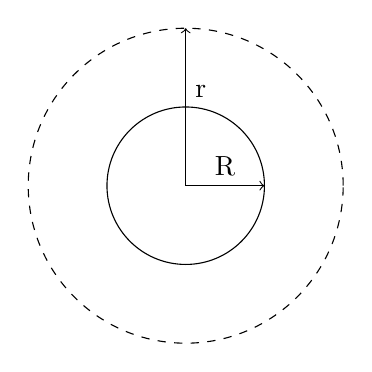
\begin{tikzpicture}
\draw (0, 0) circle(1);
\draw[->] (0, 0) -- (1, 0);
\draw (0.5, 0) node[anchor=south]{R};

\draw[dashed] (0, 0) circle(2);
\draw[->] (0, 0) -- (0, 2);
\draw (0, 1) node[anchor=south west]{r};

\end{tikzpicture}


\begin{equation}
\begin{split}
\diverg \ \grad \varphi = f
\end{split}
\end{equation}

Na rovnici aplikujeme Gaussův teorém.

\begin{equation}
\begin{split}
\int_V f \ ds = \int_V \diverg \ \grad \varphi \ ds = \int_{\partial V} (\grad \varphi) \cdot \vect{n} \ ds
\end{split}
\end{equation}

Protože potenciál závisí pouze na \(r\), tak složka gradientu kolmá na poloměr je nulová. Proto \((\grad \varphi) \cdot \vect{n} = \frac{d \varphi}{dr}\).
Získáme tak rovnici \eqref{eq:potencial_koule_obecne}.

\begin{equation}
\label{eq:potencial_koule_obecne}
\begin{split}
\int_V f \ ds = \int_{\partial V} \frac{d \varphi}{dr} \ dl = 4 \pi r^2 \frac{d \varphi}{dr}
\end{split}
\end{equation}

Označme celkové buzení \(F = \frac{4}{3} \pi R^3 f\).
Potenciál uvnitř a vně koule vyřešíme odděleně.

\subsection{Potenciál vně koule}

Tato situace nastává pokud \(r \geq R\). Uvnitř objemu \(V\) se proto nachází celá koule. Rovnici \eqref{eq:potencial_koule_obecne} proto můžeme updavit na tvar \eqref{eq:potencial_koule_vne_0}.

\begin{equation}
\label{eq:potencial_koule_vne_0}
\begin{split}
F = 4 \pi r^2 \frac{d \varphi}{dr}
\end{split}
\end{equation}

To je obyčejná diferenciální rovnice se separovatelnými proměnnými:

\begin{equation}
\label{eq:potencial_koule_vne_1}
\begin{split}
d \varphi = \frac{F}{4 \pi r^2} dr \\
\int d \varphi = \int \frac{F}{4 \pi r^2} dr \\
\varphi = -\frac{F}{4 \pi r} + C_1 \\
\end{split}
\end{equation}

Konstantu \(C_1\) jsme zvolíme 0 a získáme tak rovnici \eqref{eq:potencial_kould_vne_2}. Touto volbou zajistíme, že potenciál v nekonečnu je nulový. Konstantu lze ale zvolit jakkoli. Rovnici \eqref{eq:potencial_kould_vne_2} můžeme využít i pro bodový zdroj, kdy \(R \rightarrow 0\).

\begin{equation}
\label{eq:potencial_koule_vne_2}
\varphi = -\frac{F}{4 \pi r}
\end{equation}

\subsection{Potenciál uvnitř koule}

Tato situace nastává pokud \(r \leq R\). Uvnitř objemu \(V\) se proto nachází pouze část koule - celý objem je vyplněn koulí.

Vyjádříme \(f\) podle \(F\).

\begin{equation}
f = \frac{3}{4 \pi R^3}
\end{equation}

Integrál na levé straně rovnice \eqref{eq:potencial_koule_obecne} nahradíme vztahem pro objem koule a dosadíme za \(f\).

\begin{equation}
\begin{split}
\frac{4}{3} \pi r^3 f = 4 \pi r^2 \frac{d \varphi}{dr} \\
\frac{4}{3} \pi r^3 \frac{3}{4 \pi R^3} F = 4 \pi r^2 \frac{d \varphi}{dr} \\
\frac{r^3}{R^3} F = 4 \pi r^2 \frac{d \varphi}{dr} \\
\frac{r}{R^3} F = 4 \pi \frac{d \varphi}{dr}
\end{split}
\end{equation}

To je obyčejná diferenciální rovnice se separovatelnými proměnnými:

\begin{equation}
\label{eq:potencial_disku_uvnitr}
\begin{split}
d \varphi = \frac{r}{4 \pi R^3} F \ dr \\
\varphi = \frac{r^2}{8 \pi R^3} F + C_2
\end{split}
\end{equation}

Konstantu \(C_2\) určíme tak, aby potenciál na okraji koule (\(r = R\)) navazoval na potenciál vně koule:

\begin{equation}
\begin{split}
\frac{R^2}{8 \pi R^3} F + C_2 = -\frac{F}{4 \pi R} \\
C_2 = -\frac{F}{4 \pi R} - \frac{R^2}{8 \pi R^3} F \\
C_2 = -F \cdot \frac{3}{8 \pi R}
\end{split}
\end{equation}

Potenciál uvnitř koule je tedy

\begin{equation}
\begin{split}
\varphi = \frac{r^2}{8 \pi R^3} F - F \cdot \frac{3}{8 \pi R} \\
\varphi = \frac{F}{8 \pi R} \cdot \left(\frac{r^2}{R^2} - 3 \right) \\
\end{split}
\end{equation}

\section{Indukčnost toroidní cívky}

Toroidní cívka je cívka s jádrem ve tvaru prstence. Průřezem tohoto prstence je obvykle kruh, ale může být i jiný. Na tomto jádru je navinuto jedno nebo více vinutí. Předpokládáme,
že závity vinutí jsou kladeny rovnoměrně a dostatečně hustě na to, aby bylo možné vinutí považovat za objemový proud. Chceme určit vzájemnou indukčnost mezi dvěma cívkami s \(N_1\)
a \(N_2\) závity. Pokud bychom chtěli spočítat vlastní indukčnost, tak zvolíme \(N_1 = N_2\). Cívky jsou navinuty na jádru o obsahu průřezu \(S\) a permeabilitě \(\mu\).

Předpokládáme, že cívkou \(L_1\) s \(N_1\) závity protéká proud \(I\). Nejdříve určíme intenzitu magnetického pole \(H\) na prstenci o poloměru \(r\), který obepíná \(N_1\) závitů cívky.

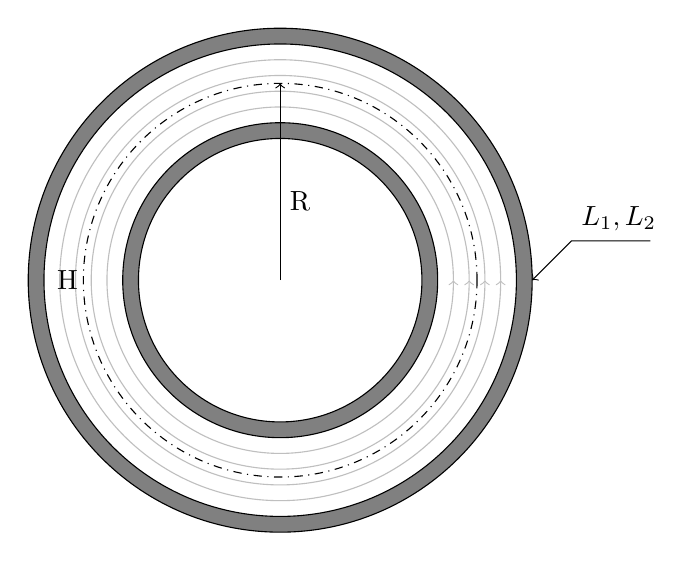
\begin{tikzpicture}
\label{img:mg_pole_toroidu}

\filldraw[color=black, fill=gray] (0, 0) circle[radius=3.2];
\filldraw[color=black, fill=white] (0, 0) circle[radius=3];

\filldraw[color=black, fill=gray] (0, 0) circle[radius=2];
\filldraw[color=black, fill=white] (0, 0) circle[radius=1.8];

\foreach \r in {2.2, 2.4, 2.6, 2.8}
	\draw[->, color=lightgray] (\r, 0) arc (0:360:\r);

\draw[dashdotted] (0, 0) circle[radius=2.5];

\draw[->] (0, 0) -- (0, 2.5);
\draw (0, 1) node[anchor=west]{R};

\draw[->] (4.7, 0.5) -- (3.7, 0.5) -- (3.2, 0);
\draw (3.7, 0.5) node[anchor=south west]{\(L_1, L_2\)};

\draw (-2.7, 0) node[anchor=center]{H};

\end{tikzpicture}

Vyjdeme z Ampérova zákona zapsaného v rovnici \eqref{eq:toroid_1}.

\begin{equation}
\label{eq:toroid_1}
\oint_{\partial P} \vect{H} \cdot d\vect{l} = \int_P \vect{j} \cdot \vect{n}
\end{equation}

Nás zajímá složka intenuity magnetického pole ve směru prstence. Označme ji \(H\). Ostatní složky jsou nulové, ale i kdyby nebyli, tak nebudou přispívat k magnetické indukci. Díky rotační symetrii je po celé délce prstence
intenzita magnetického pole stejná. Proto můžeme levou stranu rovnice \eqref{eq:toroid_1} vypočítat pomocí obvodu kruhu. Pravá strana rovnice je rovna součinu proudu a počtu závitů které prstenec obepíná.
Uvedenými úpravami získáme rovnici \label{eq:toroid_2}. Z ní lze intenzitu magnetického pole vypočítat podle vztahu \eqref{eq:toroid_3}.

\begin{equation}
\label{eq:toroid_2}
2 \pi r H = N_1 I_1
\end{equation}

\begin{equation}
\label{eq:toroid_3}
H = \frac{N_1 I_1}{2 \pi r}
\end{equation}

Pouze prstence uvnitř cívky \(L_1\) obepínají nenulový počet závitů. Vně cívek, potažmo jádra, je proto intenzita magnetického pole nulová. To je na toroidních cívkách výhodné, magnetické pole neuniká
vně cívky a naruší případné okolní obvody.

Celkový magnetický indukční tok jádrem je pak dán vztahem \eqref{eq:toroid_4}.

\begin{equation}
\label{eq:toroid_4}
\Phi = \int_S B d\vect{s} = \int_S \mu H d\vect{s} = \int_S \frac{\mu N_1 I_1}{2 \pi r} d\vect{s}
\end{equation}

Průměr prstence \(r\) se obecně mění s polohou v jádře. Je-li poloměr prstence dostatečně velký oproti rozměrům průřezu, pak jej můžeme považovat za konstantní a nahradit jej středním poloměrem prstence \(R\).

\begin{equation}
\label{eq:toroid_5}
\Phi \approx \frac{\mu N_1 I_1 S}{2 \pi R}
\end{equation}

Tento magnetický indukční tok prochází \(N_2\) závity cívky \(L_2\). Proto magnetický indukční tok, který prochází plochou obepnutou cívkou \(L_2\) je určen vztahem \eqref{eq:toroid_6}.

\begin{equation}
\label{eq:toroid_6}
\Phi_2 = N_2 \Phi \approx \frac{\mu N_1 N_2 I S}{2 \pi R}
\end{equation}

Vzájemná indukčnost je pak určena vztahem \eqref{eq:toroid_7}.

\begin{equation}
\label{eq:toroid_7}
M_{12} = \frac{\Phi_2}{I_1} \approx \frac{\mu N_1 N_2 S}{2 \pi R}
\end{equation}

